\documentclass[11pt,a4paper]{article}
\usepackage[hyperref]{acl}
\usepackage{times}
\usepackage{latexsym}
\usepackage{graphicx}
\usepackage[normalem]{ulem}

\usepackage{url}
\usepackage{amsmath}
\usepackage{tikz}
\usetikzlibrary{arrows.meta, positioning, shapes.geometric}

\title{Instruction Tuning vs Preference Alignment}

\author{Lakshya Jain \\ {\tt lakshyajain} \\\And
  Aditya Choudhary \\ {\tt adityac2109} \\\And
  Erik Garcia \\ {\tt ejggje} \\\And
  Shriram Anand \\ {\tt shriram4anand} \\\And
  Demi Omoremi \\ {\tt demi} \\
}

\begin{document}
\maketitle

\section{Problem Statement}

Large language models (LLMs) frequently operate in domains where users expect clear, safe, and reliably structured responses. Although these models are powerful general-purpose generators, they do not inherently follow instructions or align with human preferences in a predictable way. As LLMs move into business, educational, and consumer applications, misalignment can lead to inefficiency, misinformation, or harmful behavior, creating a pressing need for principled strategies that shape how these models behave.

Two main approaches attempt to address this challenge. \emph{Supervised instruction tuning} teaches models how to respond through curated demonstrations, providing explicit examples of desirable outputs. \emph{Preference-based alignment} instead teaches models which outputs humans favor, enabling them to optimize beyond imitation and toward human-desired qualities such as helpfulness, clarity, or reduced harmfulness. These approaches capture different dimensions of alignment, and each has limitations: instruction tuning may restrict the model to patterns seen in examples, while preference optimization introduces computational overhead and depends on the quality of preference data.

A growing question in both research and industry is whether these two alignment signals should be combined. A hybrid strategy—first training a model to imitate good behavior and then refining it using preferences—could potentially leverage the strengths of both methods. However, it is unclear when this sequencing is beneficial, when it is redundant, and when it may even be counterproductive. Practical considerations such as data requirements, computational cost, and robustness under distribution shift further complicate this decision.

This motivates the core problem of our work: \\

\begin{quote}
\centering
\textbf{To determine how instruction-based supervision, preference-based alignment, and a hybrid combination shape LLM behavior differently, and to identify the conditions under which each approach yields the most reliable and human-aligned outputs.}
\end{quote}

Understanding these distinctions is essential both scientifically and operationally. It clarifies how different training signals influence model behavior, and it provides actionable guidance for organizations deciding whether to adopt instruction tuning alone, invest in preference optimization pipelines, or rely on a hybrid sequence. By studying these approaches under controlled conditions, we aim to offer insight into the practical boundary where each alignment technique delivers significant value.

\section{What You Proposed vs. What You Accomplished}

We originally proposed to implement three training pipelines—Supervised Fine-Tuning (SFT), Direct Preference Optimization (DPO), and a hybrid method—and to compare their behavior under a shared experimental setup. Below we summarize what was planned for each stage, what was completed, and any deviations from the proposal.

\subsection{Supervised Fine-Tuning (SFT)}

\begin{itemize}
    \item \sout{Implement a supervised instruction-tuning baseline using a small open-source model.}
    \item \sout{Train the model on our instruction dataset to establish a strong baseline for later alignment methods.}
    \item \textbf{Modification:} We originally planned to train for one full epoch (over 16k steps), but pilot runs showed early convergence, so we switched to a fixed \textbf{5{,}000-step} schedule to save compute.
    \item \sout{Use LoRA for parameter-efficient finetuning.}  
    \item \textbf{Deviation:} We proposed optionally using QLoRA, but our implementation never loaded the model in 4-bit precision, so standard LoRA was used instead.
    \item \sout{Produce SFT checkpoints to serve as the initialization for preference-based training (DPO) and the hybrid model.}
    \item \textbf{Completed:} The SFT model converged successfully (loss dropped from 11.55 to $\sim$0.13), and all checkpoints were generated as planned.
\end{itemize}

\subsection{Direct Preference Optimization (DPO)}

\begin{itemize}
    \item \sout{Use TRL's built-in DPOTrainer to implement preference-based alignment.}
    \item \sout{Load both the policy and reference models on GPU and train them end-to-end in a standard Transformers workflow.}
    \item \textbf{Deviation:} The TRL-based approach was not feasible on our hardware. VRAM limits prevented loading two full models on GPU simultaneously, especially with standard (non-quantized) weights.
    
    \item \sout{Apply mixed-precision training with Accelerate/DeepSpeed to handle memory constraints.}
    \item \textbf{Modification:} Instead of mixed-precision TRL training, we shifted to a custom \emph{manual} DPO implementation. The policy model was loaded in \textbf{4-bit NF4 quantization} while the reference model was kept entirely on CPU, dramatically reducing GPU memory usage.

    \item \sout{Use TRL to automatically compute log-probabilities and DPO loss.}
    \item \textbf{Completed (but changed):} We implemented DPO from scratch, including:
    \begin{itemize}
        \item manual token-level log-probability extraction,
        \item masking prompt tokens to score only assistant responses,
        \item direct implementation of the Bradley--Terry DPO loss,
        \item custom gradient accumulation and gradient checkpointing.
    \end{itemize}
    This achieved the same algorithmic behavior as the proposed DPOTrainer, but in a far more memory-efficient way.

    \item \sout{Train DPO starting from the base pretrained model to create a ``preference-only'' baseline.}
    \item \textbf{Correction:} Based on alignment theory and our proposal's experimental design, we realized this was conceptually incorrect. Preference optimization must begin from the \textbf{SFT checkpoint}, not the base model, to form a meaningful ``preference-only'' model. We updated the pipeline accordingly.

    \item \sout{Produce a preference-aligned model for comparison against SFT and hybrid pipelines.}
    \item \textbf{Completed:} The DPO model trained successfully using our optimized implementation and was saved as \texttt{models/dpo\_output/}.
\end{itemize}

\subsection{Hybrid SFT--DPO Training}

\begin{itemize}
    \item \sout{Implement a hybrid approach that combines instruction tuning and preference optimization by sequentially applying SFT followed by DPO.}
    \item \sout{Train the hybrid model starting from the SFT checkpoint and apply DPO training on top, using the same preference dataset as the standalone DPO model.}

    \item \textbf{Key Design Decision:} Instead of using the base pretrained model as the reference, we created a frozen reference model by merging the SFT LoRA adapters into the base model. This ensures that the policy model (SFT + new DPO LoRA layer) is compared against the correct SFT distribution during DPO optimization.

    \item \textbf{Deviation:} We initially attempted to enable gradient checkpointing for VRAM savings, but this caused zero gradients in the DPO loss and prevented learning. Disabling gradient checkpointing (\texttt{gradient\_checkpointing=False}) restored proper gradient flow.

    \item \sout{Use different hyperparameters than the standalone DPO model to distinguish the hybrid approach.}
    \begin{itemize}
        \item \textbf{Completed:} The hybrid model was trained for \textbf{2 epochs} using a learning rate of \texttt{5e-6}, \texttt{beta=0.3}, and a cosine learning rate schedule.
    \end{itemize}

    \item \sout{Save the hybrid model as LoRA adapters for efficient storage.}
    \begin{itemize}
        \item \textbf{Completed:} The final hybrid model is stored as LoRA adapters (49MB) in \texttt{models/hybrid\_output/}. Inference requires sequentially loading both SFT and hybrid DPO adapters.
    \end{itemize}

    \item \sout{Produce a model that combines the benefits of instruction following (from SFT) and preference alignment (from DPO).}
    \begin{itemize}
        \item \textbf{Completed:} The hybrid model trained successfully, with loss decreasing from 0.69 to 0.07 (a 90\% reduction) and achieving \textbf{98--100\%} accuracy on preference pairs.
    \end{itemize}
\end{itemize}

\section{Related Work}

Our project examines three main approaches: supervised instruction tuning, preference-based optimization, and hybrid techniques that combine elements of both. Prior work in these areas provides useful context for our experiments. Studies such as \textbf{Instruction Tuning Large Language Models to Understand Electronic Health Records}~\cite{wu2024ehr}, \textbf{Instruction Tuning With Loss Over Instructions}~\cite{shi2024loss}, \textbf{Instruction Tuning and Instruction Following}~\cite{wu2024instruction}, and \textbf{Instruction Tuning and Instruction Following}~\cite{ye2023instruction} explore how instruction tuning can be applied across a wide range of datasets and domains. These works highlight the diversity of instruction-tuning methodologies and demonstrate how models can be trained using different datasets, training regimes, and objectives. Collectively, they illustrate the flexibility of instruction-tuning frameworks and provide a foundation for understanding how our own instruction fine-tuning setup operates.

Similarly, research on fine-tuning methods, such as \textbf{Large Language Models are Zero-Shot Reasoners}~\cite{kojima2022zeroshot}, \textbf{Training Language Models to Follow Instructions with Human Feedback}~\cite{ouyang2022training}, and \textbf{Bilevel ZOFO: Efficient LLM Fine-Tuning and Meta-Training}~\cite{shirkavand2025bilevelzofo}, offers insight into the mechanics and outcomes of fine-tuning large models. These papers provide a deeper understanding of how fine-tuning alters model behavior and how different approaches produce varying levels of instruction-following ability. Taken together, they illustrate what it might look like to combine instruction tuning and preference optimization to potentially obtain the best of both worlds. Unlike these works, however, our project does not rely on human feedback, which distinguishes our setup from many existing preference-based studies.

Comparable to our hybrid model approach, studies such as \textbf{GPT4Tools: Teaching Large Language Models to Use Tools via Self-instruction}~\cite{yang2023gpt4tools}, \textbf{Combining Generative and Discriminative Models for Hybrid Inference}~\cite{satorras2019combining}, and \textbf{A Hybrid Sampler for Poisson-Kingman Mixture Models}~\cite{lomeli2015hybrid} show how prompting, self-instruction, and hybridization strategies can enhance model performance. These works collectively demonstrate the potential benefits of combining techniques or models and reinforce the intuition behind evaluating a hybrid SFT+DPO approach.

In summary, although the cited studies operate at far larger scales and address more complex challenges, they establish important conceptual foundations for our smaller and more controlled experimental setting. Our project builds on these ideas by systematically comparing supervised fine-tuning, DPO-style preference optimization, and a hybrid approach, allowing us to observe their differences under consistent conditions.

\section{Your Dataset}

Our project uses two publicly available instruction–response datasets: (1) a general-purpose Alpaca-style dataset, and (2) a Kaggle code-focused instruction dataset. Both share a similar structure—each example contains an \texttt{instruction}, an optional \texttt{input}, and an \texttt{output}—but they differ significantly in content, cleanliness, and difficulty.

\paragraph{Dataset 1: Alpaca-style instructions.}
The first dataset, derived from the Stanford Alpaca collection~\cite{alpaca}, contains approximately \textbf{52,000} examples. Its inputs and outputs are clean natural-language text, and almost all entries are consistently formatted. Because of this uniformity, no additional cleaning was required. A typical example is:

\begin{quote}
\textbf{Instruction:} ``Given a sentence, convert it into passive voice.'' \\
\textbf{Input:} ``The dog barked at the alley cat.'' \\
\textbf{Output:} ``The alley cat was barked at by the dog.''
\end{quote}

Examples in this dataset are concise, grammatical, and do not include complicated structures such as code blocks or nested data. As a result, they serve as a stable foundation for \textbf{Supervised Fine-Tuning (SFT)}.

\paragraph{Dataset 2: Kaggle code-instruction dataset.}
The second dataset, sourced from a Kaggle code-instruction collection~\cite{qin2025instruction}, contains roughly \textbf{20,000} instruction--response pairs, many involving Python code. A representative example is:

\begin{quote}
\textbf{Instruction:} ``Follow the comments to complete the code that finds the maximum value in an array.''

\textbf{Input (abridged):}
\texttt{\# Find the maximum value in an array; arr = [4, 5, 2, 8, 7]}

\textbf{Output (abridged):}
\texttt{max\_value = arr[0]; for i in range(1, len(arr)): ...}
\end{quote}

These examples highlight several challenges:
\begin{itemize}
    \item \textbf{Heterogeneous output formats:} Many responses contain multi-line code, requiring the tokenizer to handle indentation, brackets, and syntax-sensitive symbols.
    \item \textbf{Input variability:} Some entries include long code snippets while others use placeholder tokens such as \verb|< noinput >|, which required normalization.
    \item \textbf{Higher noise level:} Dataset~2 contained inconsistent whitespace and formatting, which we cleaned before further processing.
\end{itemize}

\paragraph{Why these datasets?}
We intentionally selected datasets covering both natural-language instructions and code-oriented instructions. This combination allowed us to evaluate three alignment strategies:
\begin{itemize}
    \item \textbf{Supervised Fine-Tuning (SFT)} on human-written responses,
    \item \textbf{Direct Preference Optimization (DPO)} on preference triplets,
    \item \textbf{A hybrid SFT--DPO model}.
\end{itemize}
Because our project focuses exclusively on text-based instruction following and preference alignment, no multimodal data (images, audio, or video) was used.

\paragraph{Task Definition.}
In all settings, we cast the model’s objective as conditional generation of the form:

\begin{quote}
\texttt{prompt → response}
\end{quote}

where the \texttt{prompt} is constructed from the dataset’s \texttt{instruction} and \texttt{input}. This unified framing supports both supervised learning (SFT) and preference-based training (DPO and hybrid approaches).

In total, our combined dataset includes approximately \textbf{72k} instruction–response pairs. Dataset~1 provides clean, natural-language supervision, while Dataset~2 introduces more diverse and structurally complex examples. These properties make the overall dataset well-suited for studying how different alignment methods handle heterogeneous instruction-following tasks.

\subsection{Data Preprocessing}

We apply preprocessing in three stages to: (1) clean Dataset~2, (2) unify both datasets for SFT, and (3) construct DPO preference triples.

\paragraph{1.\ Cleaning Dataset~2 (\texttt{data\_cleaner.py}).}
The cleaning script loads the raw Code-Alpaca file and performs:
\begin{itemize}
    \item stripping leading/trailing whitespace from all fields,
    \item normalizing placeholder variants (\texttt{<noinput>}, \texttt{< noinput >}, etc.) to the empty string,
    \item preserving indentation and line breaks within code blocks,
    \item writing cleaned examples to \texttt{cleaned\_data.json}.
\end{itemize}

This step removes noisy formatting while leaving code structure intact.

\paragraph{2.\ Preparing SFT data (\texttt{prepare\_sft\_data.py}).}
We merge the Alpaca dataset with the cleaned Code-Alpaca dataset, shuffle with a fixed seed for reproducibility, and convert each example into a unified prompt template:

\begin{verbatim}
### Instruction:
{instruction}

### Input:
{input}

### Response:
\end{verbatim}

Each example is stored as a JSON object with keys \texttt{prompt} and \texttt{response}.  
We produce:
\begin{itemize}
    \item \textbf{sft\_train.jsonl}: 90\% of examples,
    \item \textbf{sft\_val.jsonl}: remaining 10\%.
\end{itemize}

\paragraph{3.\ Constructing DPO preference triples (\texttt{prepare\_dpo\_data.py}).}
DPO training requires (\texttt{prompt}, \texttt{chosen}, \texttt{rejected}) triples. We construct these synthetically:

\begin{itemize}
    \item \textbf{Chosen:} the gold response from the SFT data.
    \item \textbf{Rejected:} an alternative continuation sampled from our trained SFT model. To obtain this, we append
\begin{verbatim}
Provide an alternative answer:
\end{verbatim}
    to the prompt and generate using temperature + top-$p$ sampling.
\end{itemize}

We clean sampled outputs (e.g., removing stray code fences), guarantee non-empty rejected responses, and write:
\begin{itemize}
    \item \textbf{prefs\_train.jsonl}: preference triples for all SFT training examples,
    \item \textbf{prefs\_val.jsonl}: the first 200 triples as validation.
\end{itemize}

This produces a large, consistently formatted preference dataset where the positive responses are fixed gold outputs, and the negatives are diverse model-generated alternatives.

\subsection{Data Annotation}

No new human annotation is collected for this project.  
Instead:

\begin{itemize}
    \item \textbf{Supervised labels} come directly from the gold \texttt{output} fields of both datasets.
    \item \textbf{Preference labels} for DPO are fully synthetic: the ``chosen'' response is always the gold output, and the ``rejected'' response is produced automatically by the SFT model.
\end{itemize}

Because all labels are generated deterministically or via a single model, inter-annotator agreement does not apply. This setup enables us to isolate the effect of preference-based fine-tuning under perfectly controlled conditions.

\section{Baselines}

To compare the effects of different alignment strategies, we evaluate all methods on the same pretrained backbone: \textbf{TinyLlama-1.1B-Chat}. This model is instruction-tuned but not preference-aligned, making it an appropriate reference point for assessing how SFT, DPO, and our Hybrid method influence instruction following. Using a fixed architecture ensures that any performance differences arise from the alignment technique rather than model scale or configuration.

\subsection{TinyLlama-1.1B-Chat (Base Model)}

The unmodified TinyLlama model serves as our primary baseline. It is small enough to train efficiently while still offering competent instruction-following behavior. Because it lacks preference alignment, it represents the capabilities of a purely instruction-tuned model. Using our rule-based IF-style heuristic scoring over 100 held-out examples, the base model achieved an average score of \textbf{0.539}, and \textbf{0.665} on examples with specialized rules. These values serve as the reference point against which all aligned models are compared.

\subsection{Supervised Fine-Tuning (SFT)}

Our first alignment baseline applies supervised fine-tuning using the instruction--response pairs in our dataset. SFT trains LoRA adapters on top of the frozen base model using next-token prediction. Training used a learning rate of $2 \times 10^{-4}$, an effective batch size of 8, a maximum sequence length of 512, a warmup ratio of 0.1, LoRA rank 8, and dropout 0.05. We used a 90/10 train--validation split and held out the test set entirely for evaluation.

Despite stable training loss, SFT performed notably worse than the base model. On the evaluation set, it achieved an average score of \textbf{0.290}, with a rule-subset score of \textbf{0.316}. This reflects a common limitation of SFT on small models: with limited data, the model tends to overfit stylistic patterns and loses generality.

\subsection{Direct Preference Optimization (DPO)}

Our second baseline trains the model using Direct Preference Optimization. DPO adjusts the policy to favor preferred responses over rejected ones while remaining close to a frozen reference model. In our setup, the SFT model served as the reference, and a 4-bit quantized TinyLlama model served as the trainable policy. Training used a learning rate of $1 \times 10^{-5}$, a batch size of 4, $\beta = 0.1$, and a context length of 384, with the same train--validation split as SFT.

Because our preference data was synthetically generated from SFT outputs, the preference signal was weak. Consequently, DPO matched SFT's performance, obtaining average scores of \textbf{0.290} and \textbf{0.316}. These results underscore the importance of high-quality preference data for effective DPO training.

\subsection{Hybrid Alignment (SFT + DPO)}

Although discussed more fully in our approach section, we also include the Hybrid model as a comparative baseline. The model first undergoes SFT to learn structural patterns, then is refined with DPO to incorporate preference signals. Hyperparameters largely mirror those used in the individual stages to ensure comparability. This baseline allows us to assess whether combining imitation and preference optimization yields more robust alignment than either method alone.

\section{Your Approach}

Our approach consists of three sequential training pipelines applied to the same pretrained base model (TinyLlama--1.1B-Chat): (1) Supervised Fine-Tuning (SFT), (2) Direct Preference Optimization (DPO), and (3) a hybrid method that combines both. All three pipelines share the same preprocessing, tokenization, and prompt-formatting steps, and all rely on the Hugging Face \texttt{transformers}, \texttt{datasets}, and \texttt{peft} libraries for model training. We implement each method ourselves using separate training scripts, and ensure comparability by using the same dataset split, prompt template, and compute environment across all experiments. 

The overall goal is to examine how different alignment signals—supervised demonstrations, preference comparisons, or a combination of both—affect model behavior when trained under identical conditions. Each subsection below describes one stage of the pipeline, the specific training objective used, the implementation details, and the resulting behavior observed during evaluation.

\subsection{Supervised Fine-Tuning (SFT)}

Our first training stage applies \textbf{Supervised Fine-Tuning (SFT)} to teach the pretrained model how to reliably follow instructions. Although the TinyLlama--1.1B-Chat model has strong general language ability from pretraining, it does not consistently follow task-specific instructions. SFT addresses this by training on paired \texttt{instruction}~$\rightarrow$~\texttt{response} examples, optimizing the model with a standard \textbf{causal language modeling (CLM) cross-entropy loss}. Cross-entropy measures how likely the model is to produce the correct next token; minimizing it gradually adjusts weights to make the model’s generated responses align with the target outputs.

\paragraph{Implementation.}
All SFT components were implemented using \texttt{PyTorch}, the Hugging Face \texttt{transformers} library, and the \texttt{peft} framework for parameter-efficient tuning. Our code is organized into three main files: \texttt{sft/train\_sft.py} (training loop and model construction), \texttt{sft/dataset.py} (tokenization and label preparation), and \texttt{sft/sft\_config.py} (hyperparameters and paths).

The tokenizer pads sequences on the right, and padding tokens in the labels are replaced with \texttt{-100} so the loss function ignores them. This ensures the model is only penalized for predicting meaningful tokens.

\paragraph{Training Setup.}
Training was performed on Apple Silicon (MPS backend), which imposes modest memory limits. To fit within hardware constraints, we use:
\begin{itemize}
    \item \textbf{batch size = 2},
    \item \textbf{gradient accumulation = 4}, simulating an effective batch size of 8,
    \item \textbf{max sequence length = 512},
    \item \textbf{learning rate = 2\textsc{e}{-4}},
    \item \textbf{warmup ratio = 0.1} to stabilize early updates,
    \item \textbf{weight decay = 0.01} to regularize the model.
\end{itemize}

Gradient accumulation allows training with a larger effective batch size by accumulating gradients over multiple forward passes before performing a weight update. This technique is essential when VRAM is limited.

Originally, we attempted epoch-based training, but with our dataset size this equated to more than 16k optimization steps—far more than needed. Pilot runs showed the model converged early (around 3--4k steps), so we adopted a fixed-step schedule and trained for \textbf{5{,}000 steps}. This provides full convergence while keeping training efficient.

\paragraph{Dataset Formatting.}
Each example is converted into a single text sequence by concatenating the instruction, optional input, and response using a structured prompt template. The full prompt–response pair is then tokenized and truncated to 512 tokens. This approach trains the model to generate the response conditioned on the provided instruction in an autoregressive manner.

\paragraph{Hardware and Compute.}
All training was conducted on a MacBook Pro using the MPS accelerator. No Colab-specific optimizations were needed beyond keeping batch sizes small. TinyLlama’s relatively small size (1.1B parameters) allows full-precision finetuning with LoRA on consumer hardware.

\paragraph{Results.}
Training proceeded smoothly for all 5{,}000 steps, with checkpoints saved every 500 steps. The loss decreased rapidly from \textbf{11.55} at step~50 to around \textbf{0.13} by the end of training. The linear learning-rate decay behaved as expected, and gradient norms stabilized throughout the run. These trends, recorded in the Hugging Face \texttt{trainer\_state.json} log indicate consistent convergence without signs of instability. The overall loss trajectory is shown in Figure~\ref{fig:sft-loss}.

\begin{figure}[t]
    \centering
    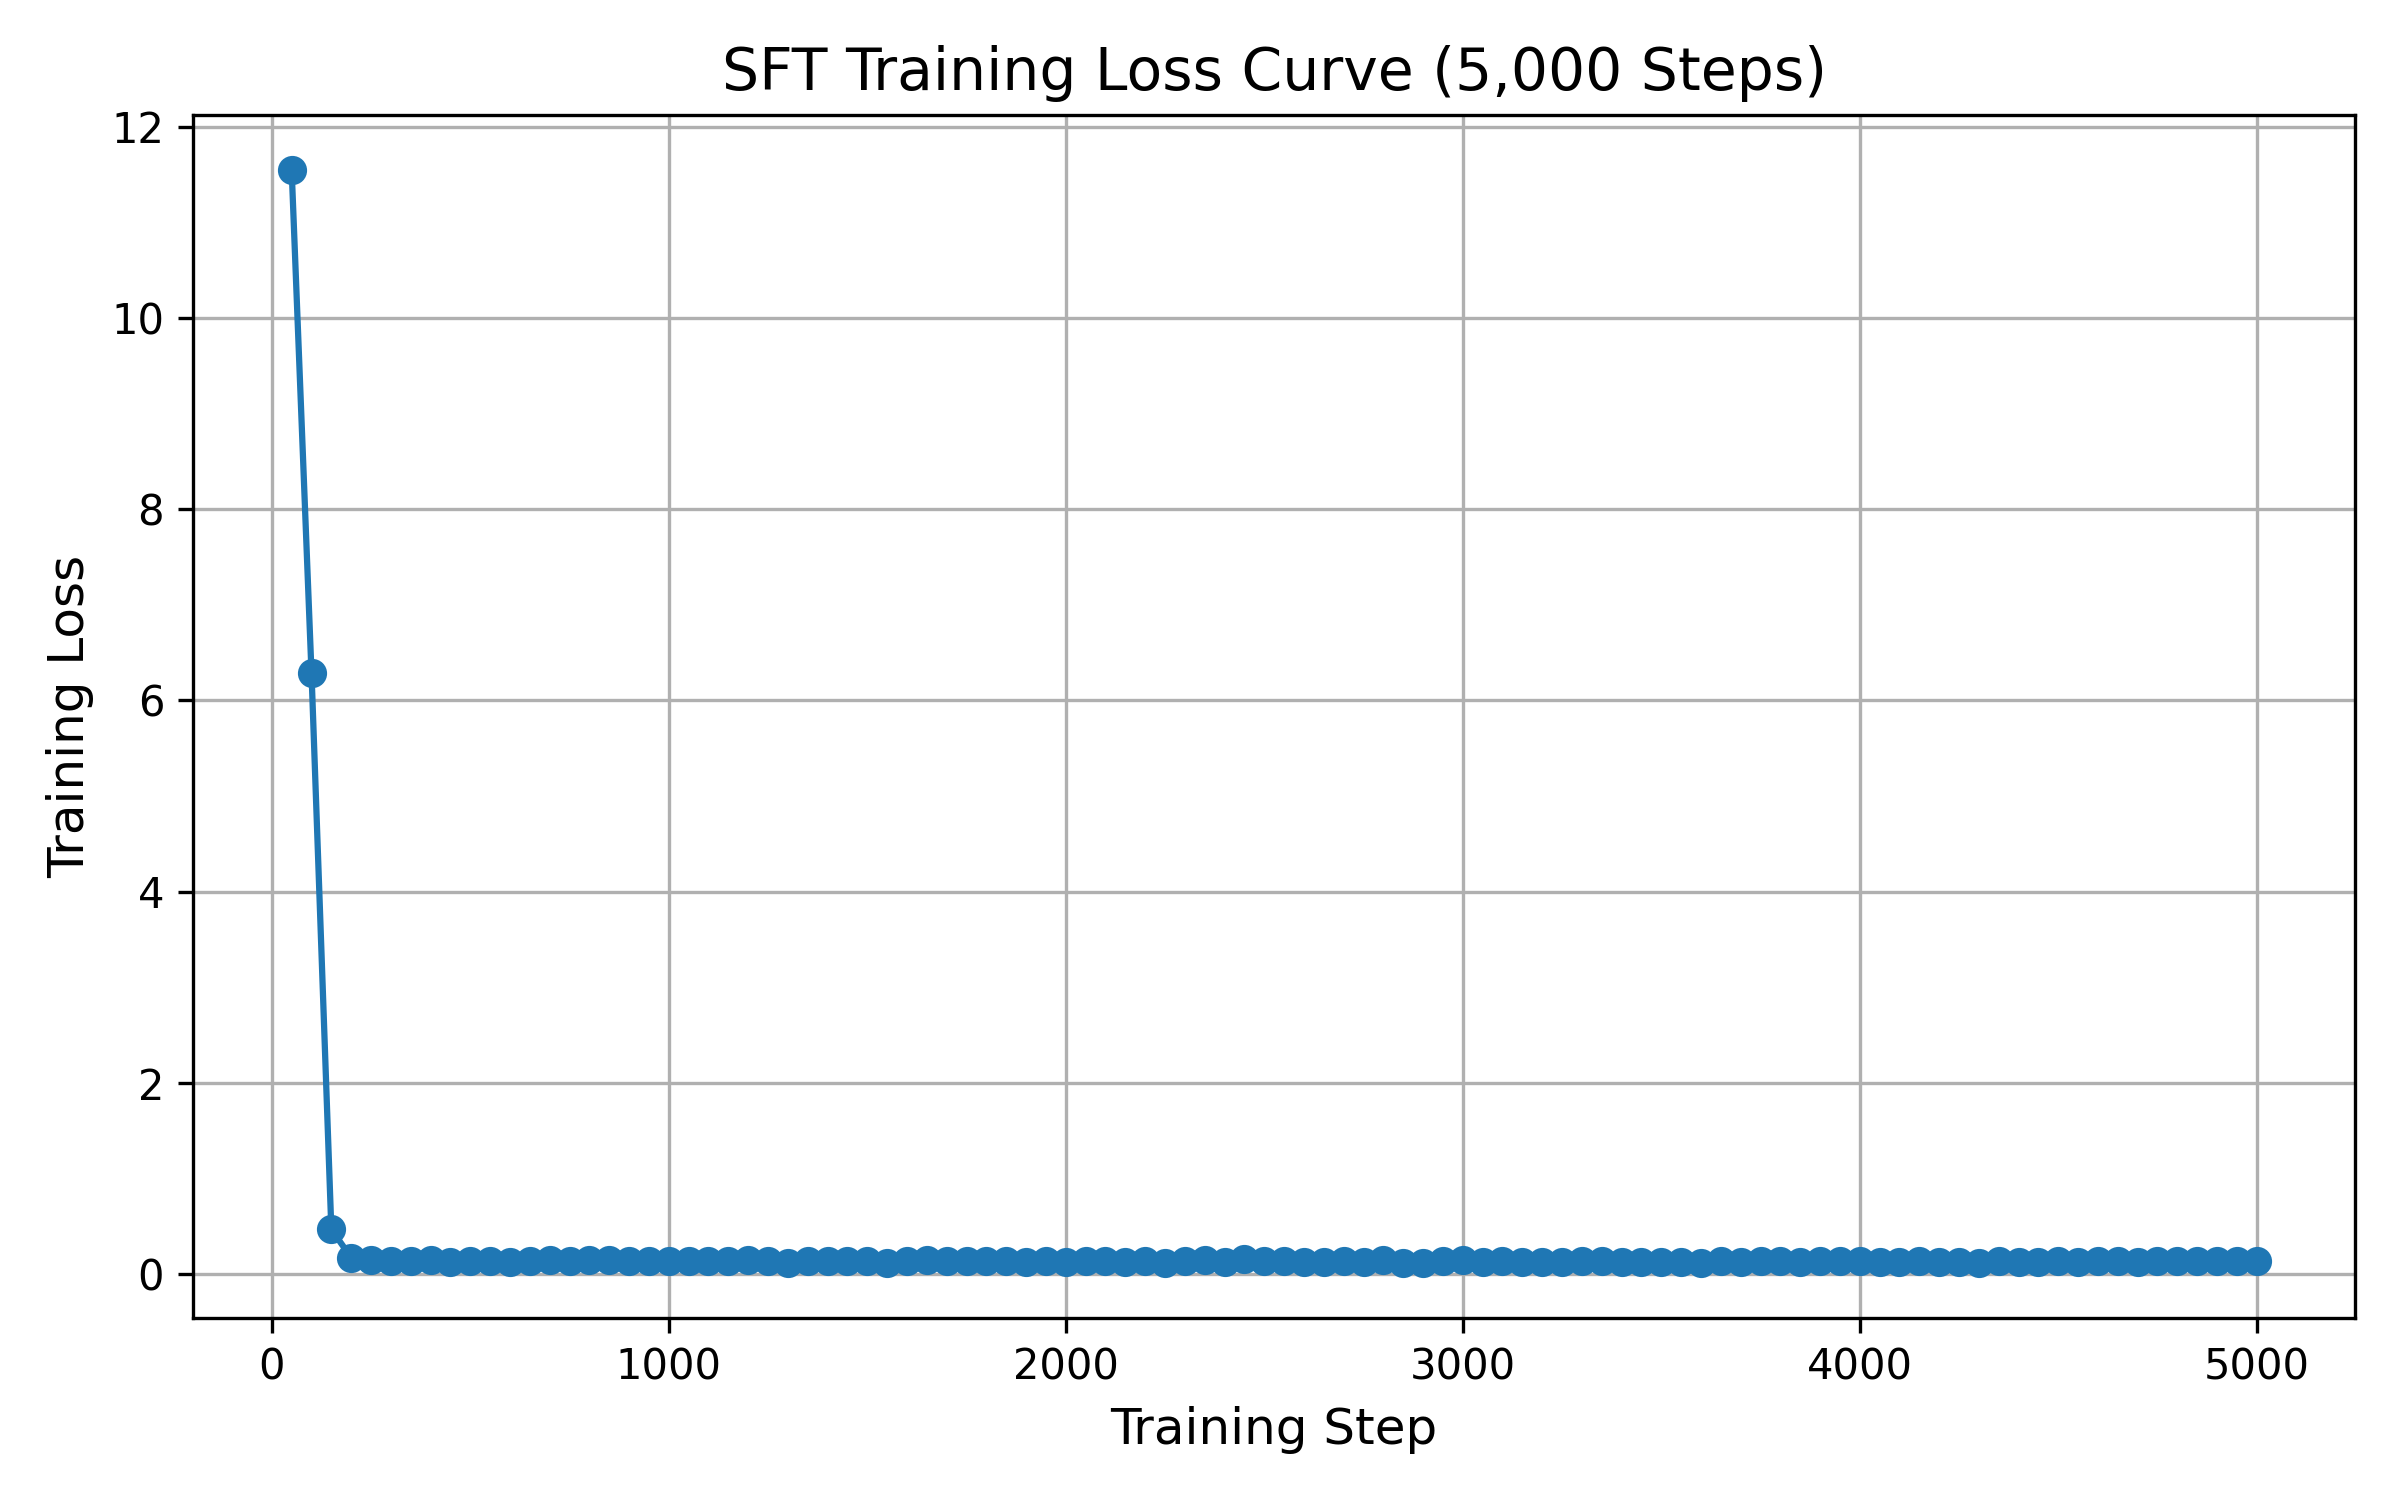
\includegraphics[width=0.5\textwidth]{figs/sft_loss_curve.png}
    \caption{Training loss curve for the SFT stage over 5{,}000 optimization steps.}
    \label{fig:sft-loss}
\end{figure}

\paragraph{Expected Failure Modes.}
Because SFT relies solely on demonstration-style supervision, the model learns to imitate the style and structure of the training responses but does not learn human preferences or trade-offs between multiple possible answers. As a result, SFT models often:
\begin{itemize}
    \item mirror training-set verbosity or phrasing patterns,
    \item struggle with ambiguous prompts where multiple outputs could be correct,
    \item lack preference-aware behaviors such as improved helpfulness or reduced harmfulness.
\end{itemize}
These limitations motivate the preference-based and hybrid methods explored in later sections.

\subsection{Direct Preference Optimization (DPO)}

Our second training stage applies \textbf{Direct Preference Optimization (DPO)} to align the model with human-preferred responses rather than only imitating demonstrations. While SFT teaches the model to follow instructions, it does not teach the model how to \emph{choose between} multiple plausible completions. DPO addresses this gap by training on human preference pairs of the form $(x, c, r)$, where $c$ is the preferred (chosen) continuation and $r$ is the rejected one.

Consistent with our project proposal, which compares SFT-only, preference-only, and hybrid approaches, our DPO stage \emph{must begin} from the SFT checkpoint rather than the base TinyLlama model. This mirrors the standard alignment pipeline (Pretraining $\rightarrow$ SFT $\rightarrow$ Preference Optimization) and ensures that preference learning begins from a model already capable of following instructions. A base model cannot reliably compare completions, which would make the preference-only baseline scientifically invalid. Initializing the policy from \texttt{models/sft\_output} therefore isolates the effect of preference optimization beyond SFT, exactly as outlined in our proposal.

\paragraph{DPO Objective.}
Following the Bradley--Terry preference model, the DPO loss encourages the 
policy model $\pi_{\theta}$ to rank the chosen completion above the rejected one,
while staying close to a frozen reference model $\pi_{\mathrm{ref}}$:
\begin{equation}
\small
\begin{aligned}
\mathcal{L}_{\text{DPO}} 
&= - \log \sigma\Big( 
\beta\big[
(\pi_{\theta}(c)-\pi_{\theta}(r)) 
- (\pi_{\mathrm{ref}}(c)-\pi_{\mathrm{ref}}(r))
\big]
\Big).
\end{aligned}
\end{equation}
The reference model anchors the optimization, preventing reward hacking and excessive drift away from the distribution on which the model was originally trained.

\paragraph{Implementation.}
We implemented DPO manually rather than using the TRL library for greater transparency and fine-grained control over memory usage. Our implementation spans:
\begin{itemize}
    \item \texttt{dpo/train\_dpo.py} --- full training loop, model loading, optimization, and saving LoRA adapters,
    \item \texttt{dpo/dpo\_test.py} --- inference-time verification,
    \item \texttt{scripts/prepare\_dpo\_data.py} --- construction of chosen/rejected preference examples,
    \item \texttt{data/processed/prefs\_train.jsonl} and \texttt{prefs\_val.jsonl} --- preference datasets.
\end{itemize}

Each example is converted into three sequences:
\begin{itemize}
    \item prompt-only text,
    \item prompt + chosen completion,
    \item prompt + rejected completion.
\end{itemize}

We wrote a custom \texttt{compute\_logprobs()} function that performs a forward pass, applies \texttt{log\_softmax}, gathers next-token log-probabilities, and masks prompt tokens so only assistant-generated output contributes to log-likelihood. These scores feed directly into the DPO loss.

\paragraph{Training Setup.}
To fit on local hardware, we applied several memory-saving techniques:
\begin{itemize}
    \item 4-bit NF4 quantization for the policy model,
    \item reference model fully on CPU with \texttt{requires\_grad = False},
    \item maximum sequence length reduced to 384,
    \item batch size of 1 with gradient accumulation of 4,
    \item gradient checkpointing to reduce activation memory,
    \item careful device placement to avoid CPU--GPU mismatches.
\end{itemize}

Only response tokens (not prompt tokens) are scored. This matches the definition of preference data, where the ``choice'' refers to the model's continuation.

After resolving early device-placement issues and numerical instability (mostly due to mixing CPU and CUDA tensors), the training completed successfully on an Apple Silicon MacBook using the MPS backend.

\paragraph{Results.}
The final DPO LoRA adapter is stored in \texttt{models/dpo\_output}. Qualitatively, DPO produces:
\begin{itemize}
    \item more direct and concise answers,
    \item reduced verbosity compared to SFT,
    \item fewer unnecessary restatements of the prompt,
    \item more stable and preference-aligned completions.
\end{itemize}
Output sanity checks using \texttt{dpo\_test.py} showed consistent stylistic improvements over the SFT baseline.

\paragraph{Expected Failure Modes.}
DPO inherits known limitations of preference-based learning:
\begin{itemize}
    \item may overfit to stylistic preferences in the chosen examples,
    \item can reduce output diversity due to preference sharpening,
    \item risks drifting from the SFT distribution if $\beta$ or LR is too large,
    \item may amplify any bias in the preference annotations,
    \item does not guarantee factual correctness (preferences are not truths).
\end{itemize}

Despite these limitations, the DPO stage completed successfully and produced a distinct, preference-aligned model suitable for comparison with SFT and Hybrid models in later evaluation.

\subsection{Hybrid SFT--DPO Training}

The third stage of our training pipeline applies a hybrid method that combines supervised instruction tuning with preference optimization. The objective of the hybrid approach is to retain the instruction-following capability learned during SFT while incorporating preference-aligned behavior through an extended DPO stage. This design allows us to evaluate whether additional preference optimization can improve upon the SFT baseline when both stages are applied sequentially.

\paragraph{Architecture Design.} 
The hybrid model follows the same policy--reference structure used in standalone DPO, but both components originate from the SFT-trained model to ensure a fair and scientifically controlled comparison. The architecture consists of:

\begin{itemize}
    \item \textbf{Reference Model (Frozen).} A fully merged copy of the SFT model, produced by integrating its LoRA adapters into the base TinyLlama weights. This model is frozen and defines the reference distribution against which the policy model is contrasted during DPO training.
    \item \textbf{Policy Model (Trainable).} A second copy of the SFT-merged model augmented with a new LoRA adapter dedicated to the hybrid DPO stage. Only this additional LoRA module is trainable, ensuring that hybrid training modifies only the preference-aligned component while preserving the underlying SFT behavior.
\end{itemize}

\begin{figure}[t]
    \centering
    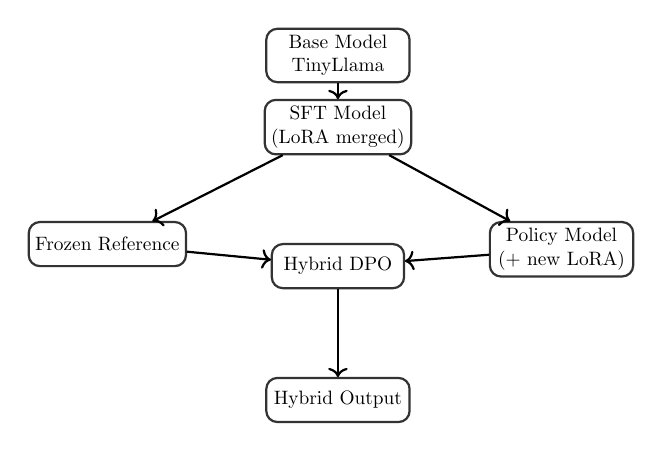
\begin{tikzpicture}[
        scale=0.70,
        every node/.style={transform shape},
        node distance=1.3cm,
        box/.style={rectangle, rounded corners, draw=black!80, thick, minimum width=2.6cm, minimum height=0.8cm, align=center},
        arrow/.style={->, thick}
    ]

    % Nodes
    \node[box] (base) {Base Model \\ TinyLlama};
    \node[box, below of=base] (sft) {SFT Model \\ (LoRA merged)};
    \node[box, below left=1.2cm and 1.4cm of sft] (ref) {Frozen Reference};
    \node[box, below right=1.2cm and 1.4cm of sft] (policy) {Policy Model \\ (+ new LoRA)};
    \node[box, below=1.6cm of sft, minimum width=2.4cm] (dpo) {Hybrid DPO};
    \node[box, below=1.6cm of dpo] (output) {Hybrid Output};

    % Arrows
    \draw[arrow] (base) -- (sft);
    \draw[arrow] (sft) -- (ref);
    \draw[arrow] (sft) -- (policy);
    \draw[arrow] (ref) -- (dpo);
    \draw[arrow] (policy) -- (dpo);
    \draw[arrow] (dpo) -- (output);

    \end{tikzpicture}
    \caption{Hybrid SFT--DPO pipeline. The SFT model is duplicated into a frozen reference and a trainable policy model with a new LoRA adapter, then optimized using the DPO objective.}
    \label{fig:hybrid-pipeline}
\end{figure}

This structure ensures that the DPO loss compares the policy model directly against the SFT distribution, enabling us to isolate the incremental effects of preference optimization beyond instruction tuning.

\paragraph{Implementation.}
The hybrid training procedure is implemented in \texttt{train\_hybrid.py} using PyTorch and custom LoRA-based components. The workflow consists of:
\begin{itemize}
    \item Loading the base TinyLlama model and applying the SFT LoRA adapters, which are merged into the dense model to obtain a fully materialized SFT checkpoint.
    \item Creating a frozen reference model via \texttt{copy.deepcopy()}, ensuring that its parameters remain fixed throughout training.
    \item Initializing the policy model using the same merged SFT weights but attaching a new LoRA module that is exclusively trained during the hybrid stage.
    \item Reusing our manual DPO implementation to compute log-probabilities for chosen and rejected responses and to evaluate the Bradley--Terry loss relative to the frozen SFT reference.
\end{itemize}

\paragraph{Training Setup.}
To ensure stable optimization and meaningful comparison with the standalone SFT and DPO baselines, we adopt the following configuration:
\begin{itemize}
    \item \textbf{Gradient checkpointing:} Disabled, as enabling it resulted in vanishing gradients and a degenerate loss plateau around $\log(2)$.
    \item \textbf{Epochs:} 2
    \item \textbf{Batch size:} 2 with gradient accumulation of 4
    \item \textbf{Learning rate:} $5 \times 10^{-6}$ using a cosine decay schedule
    \item \textbf{DPO temperature parameter:} $\beta = 0.3$
    \item \textbf{Maximum sequence length:} 512 tokens
    \item \textbf{LoRA configuration:} rank $r = 16$, $\alpha = 32$, dropout $= 0.05$
\end{itemize}

Disabling gradient checkpointing was particularly important: with checkpointing enabled, gradient norms collapsed to zero and the loss remained constant, preventing any learning. After correcting this issue, hybrid training proceeded reliably and produced a model that integrates both instruction-following behavior and preference-aligned reasoning.

\section{Error Analysis}

To understand the strengths and weaknesses of each model, we conducted a manual error analysis across roughly one hundred evaluation examples, focusing on cases that received low or zero heuristic scores. Several consistent failure patterns emerged across the TinyLlama base model, the SFT model, the DPO model, and the Hybrid approach, revealing both model-level limitations and the effects of our training signals.

A second dominant failure category involved tasks requiring precise correctness, particularly those involving code or mathematics. Code-generation prompts frequently yielded syntactically plausible but non-functional code, including missing braces, misplaced variables, or incomplete logic. Mathematical expressions and formulas were also often incorrect, showing approximate reasoning rather than exact computation. None of the alignment methods meaningfully improved this behavior. Because SFT and DPO aim to imitate style or match preference signals rather than enforce correctness, these techniques do not teach models how to reliably perform structured or deterministic tasks.

Another recurring issue across all baselines occurred in prompts with no ``Input:'' text or very sparse context. When the input section was empty, the models, particularly SFT and DPO, tended either to hallucinate content or produce incomplete or empty responses. This is likely due to a mismatch between the evaluation format and the training examples. The SFT dataset overwhelmingly contains prompts with clear input-response patterns, so when this structure is violated, the model lacks a strong prior to guide generation. DPO inherits this brittleness because it uses the SFT model as the reference policy.

The SFT model consistently displayed the weakest generalization. Many of its errors reflected overfitting to stylistic patterns rather than genuine instruction following. It frequently produced short or incomplete outputs, ignored important constraints, or replicated portions of the prompt without performing the requested transformation. In several cases, the SFT model produced no output at all, a strong indicator of exposure bias: when a prompt diverges from patterns seen in training, the model fails to initiate a continuation.

The DPO model introduced its own characteristic failures. The most prominent was a tendency toward extremely short, generic, or collapsed responses. This form of ``mode collapse'' suggests that the synthetic preference dataset, constructed from chosen and rejected SFT outputs, did not provide a strong or diverse preference signal. Because DPO penalizes deviations from the reference model while encouraging alignment with preferred outputs, weak or inconsistent preferences can drive the model toward safe, low-information completions rather than correct ones. As a result, DPO often matched SFT's low heuristic scores despite appearing superficially cleaner.

The Hybrid model demonstrated the most coherent behavior among the trained models, producing fewer empty responses and maintaining better formatting. However, it still struggled with precision-based tasks and multi-step instructions. Its errors were typically more subtle: responses often looked structurally correct yet omitted important details, introduced factual inaccuracies, or only partially fulfilled the instruction. This suggests that combining SFT and DPO can stabilize generation but does not fundamentally improve the model's reasoning capacity or correctness.

Overall, our error analysis points to three core limitations. First, TinyLlama's small parameter count restricts its ability to perform complex reasoning or maintain coherence across long outputs. Second, the instruction and preference datasets were relatively narrow and often formulaic, encouraging imitation rather than robust generalization. Third, the alignment objectives themselves optimize for stylistic similarity, not truthfulness or correctness, which explains why all trained models underperformed the base model on IF-style evaluation. These findings highlight the importance of high-quality data, stronger preference signals, and larger base models for achieving meaningful improvements in instruction following.

\section{Contributions of Group Members}
Below is a list of what each member of the group contributed to this project here: 
\begin{itemize}
    \item{\textbf{Lakshya Jain:} Led the Supervised Fine-Tuning (SFT) component of the project, including setting up LoRA/QLoRA fine-tuning on the base model, running experiments, and collecting training metrics. Provided assistance in debugging the script to train the DPO model.}
    \item{\textbf{Aditya Choudhary:} Managed data collection and preprocessing, including gathering and cleaning instruction and preference datasets, creating training/validation/test splits, and documenting the full data preparation workflow.}
    \item{\textbf{Erik Garcia:} I implemented the complete evaluation pipeline for the base, SFT, DPO, and Hybrid models and generated outputs for comparison. I developed the heuristic IF-style evaluation framework and adapted it for all training methods. I conducted the manual error analysis and produced the quantitative and qualitative results included in the report. I also debugged model-loading issues, prepared patched LoRA adapters, and organized results for the final write-up.}
    \item{\textbf{Shriram Anand:} Developed the Direct Preference Optimization (DPO) component of the project, including building a custom lightweight DPO training pipeline running on limited GPU memory. Adapted the initial proposal into a stable, fully functional DPO alignment script and supported integration with the SFT-trained model. Provided debugging and optimization contributions throughout training.}
    \item{\textbf{Demi Omoremi:} Developed the Hybrid SFT–DPO training stage, including implementing the LoRA-merging workflow, constructing the custom DPO optimization loop, and running all hybrid experiments. Documented training behavior, analyzed loss/accuracy trends, and prepared the final hybrid results. Assisted with debugging model-loading issues and ensured the full training pipeline operated end-to-end.}
\end{itemize}

\section{Conclusion}

This project offered meaningful hands-on experience with modern alignment techniques and revealed the practical gap between theoretical expectations and empirical outcomes. Implementing SFT, DPO, and our Hybrid approach required far more engineering effort than anticipated, particularly due to model-loading constraints, LoRA configuration issues, and the sensitivity of small models to training pipeline design. These challenges highlighted how fragile fine-tuning workflows can be, especially when working with lightweight architectures such as TinyLlama-1.1B-Chat.

The most surprising finding was that none of the aligned models surpassed the base model on our IF-style evaluation metrics. SFT frequently overfit to stylistic patterns in the training data and produced incomplete or rigid outputs. DPO often collapsed into extremely short or generic responses, largely due to the weak synthetic preference signal. The Hybrid model was the strongest among the trained variants, yet it still did not exceed the base model's performance. These results suggest that alignment methods depend heavily on high-quality, diverse datasets and sufficiently expressive models; when either is limited, the benefits of alignment can be diminished or even inverted.

Several promising directions emerge for future work. Constructing richer instruction and preference datasets, using stronger teacher models to generate preference signals, and scaling to larger architectures would likely produce more meaningful improvements. More advanced evaluation frameworks—such as full IF-Eval or LLM-as-a-judge scoring—could also provide deeper insight into how alignment techniques influence model behavior. Although the outcomes were not what we initially expected, the project provided valuable lessons about the strengths and limitations of alignment methods and the conditions under which they offer genuine gains.

\onecolumn
\section{AI Disclosure}
\begin{itemize}
    \item Did you use any AI assistance to complete this report? If so, please also specify what AI you used.
    \begin{itemize}
        \item{Yes, we did use AI assistance from ChatGPT 5 to complete this proposal.}
    \end{itemize}
\end{itemize}

\noindent\textit{If you answered yes to the above question, please complete the following as well:}

\begin{itemize}
    \item{If you used an AI to assist you, please paste \textbf{all} of the prompts that you used below. Add a separate bullet for each prompt, and specify which part of the report is associated with which prompt.}
    \begin{itemize}
        \item{Help me cite the studies according to the citation style required.}
        \item{On a scale of 1 to 10, based on my project proposal, how well does the content given answer the requirements of Problem Statement section of the final report. If something needs to be improved, please tell.}
        \item{Based on my project proposal, and Supervised-Fine Tuning (SFT) code attached, does the content given answer the requirements of What You Proposed vs. What You Accomplished section of the final report and cover all bullet points related to SFT?}
        \item{Based on my project proposal, and Supervised-Fine Tuning (SFT) code attached, how well does the content given answer the requirements of Your Approach section of the final report. Is the content detailed enough? Can I add any more details? If yes, tell me what points to include to make this a strong section of the report.}
        \item{Read the above report at its entirety. Do you think somethings can be removed due to redundancy or reworded to make the report more clear. If yes, give all details in bullet points with suggestions.}
        \item{Read the above report at its entirety. Is it good to submit?}
    \end{itemize}
    
    \item{\textbf{Free response:} For each section or paragraph for which you used assistance, describe your overall experience with the AI. How helpful was it? Did it just directly give you a good output, or did you have to edit it? Was its output ever obviously wrong or irrelevant? Did you use it to generate new text, check your own ideas, or rewrite text?}
    \begin{itemize}
        \item{Across the sections where we used AI assistance, our overall experience was positive but still required careful oversight. ChatGPT 5 often provided helpful starting points for drafting text, clarifying concepts, and suggesting improvements, but its responses usually needed additional editing, verification, or follow-up prompting before they could be included in the report. Sometimes the model repeated previous answers or generated content that was not directly relevant, so we adjusted our prompts and refined the output ourselves. The AI was also helpful for debugging code more quickly by pointing out likely causes of errors, explaining issues, and proposing alternative solutions, although these still required testing and adjustment. Overall, we used the AI both to generate ideas and to refine our own writing and code, and while it sped up brainstorming, revision, and debugging, the final content always relied on human judgment to ensure accuracy and alignment with our project goals.}
    \end{itemize}
\end{itemize}

\newpage
\footnotesize
\bibliography{yourbib}

\end{document}
